\section{Derivation of the algorithm}\label{sec:Implementation}
The derivation of the algorithm of the thesis is shown in this section. First, I apply the theories and methods mentioned before on the image registration process to get my algorithm. After that, the application of my algorithm to a simple case with rectified stereo images is shown. In the end, my algorithm is applied to the unrectified images i.e. arbitrary images.
\subsection{Image registration Process}
Similar images are created in many situations, such as from stereo cameras, map updating and motion detection. Image registration process can be applied on this similar images to match or register the same structure or patches in both images. And the algorithm is a kind of image registration algorithm to register the plane patches in images with the multiple homography approach.

In order to introduce the algorithm, we assume that there is a pair of images with same plane patches, which are from the stereo cameras or consecutive images from the aerial video. Let the two images be $I_1$ and $I_2$ where we call $I_1$ the "template image" and $I_2$ the "target image". The template image is is formulated as the brightness function $I_1(\rdx'_{ij})$, in which $\rdx'_{ij}$ means the pixel coordinate of the pixel at row $i$ and column $j$. And the target image is defined as $I_2(\rdy'_{ij})$, in which $\rdy'_{ij}$ means the pixel coordinate of the point in target image, which is corresponding to the point $\rdx'_{ij}$ in template image. The symbol $I_1$ and $I_2$ here represent respectively the function that can transform the coordinate variable to pixel value, i.e. $I$ transform the variable in space $\dsR^{2}$ to space $\dsR$(In the thesis, only gray-scaled images is consider for simplicity. But the generalization to color images is not complicated, applying the algorithm on three channels of the image separately and add them up finally). Further more, we will use the homography transformation per patch to do the registration separately, so function $T_n$ represents the process of homography transformation from space $\dsR^{3}$ to space $\dsR^3$ with homogeneous coordinate for plane patch $n$. Here we define $T_n$ for plane patch $n$ from template to target image.

But a problem comes now, the output of $T_n$ is a 3-length vector in $\dsR^3$ space, the input of $I_2$ is paradoxically a 2-length vector in $\dsR^2$ space. So we still need a dehomogenization function to connect them to describe the transformation process. Therefore, we introduce the function $N$ to do dehomogenization transformation:
\begin{align} \label{eq:N}
	\rdx'_{ij} = N(\rdx_{ij}) \\
	\rdy'_{ij} = N(\rdy_{ij})
\end{align}
where $\rdx_{ij}$($\rdy_{ij}$) and ${\rdx_{ij}}'$(${\rdy_{ij}}'$)  are homogeneous coordinate and Cartesian coordinate of pixel in template image(target image).

From the \cref{eq:homography_infty}, the corresponding pixels in the plane region $n$ of template and target image can be connected as:
\begin{align}
	\rdy_{ij} & = H_n \cdot \rdx_{ij} \nonumber \\
			& = (H_{\infty} + \rde \cdot \vec{q}_{n}^T) \rdx_{ij}
\end{align}	
where $\rdx_{ij} = (\rdx'_{ij}, 1)^T$ and $\rdx_{ij}$ means the $i$ row $j$ column in every patch. $H_\infty$ and $\vec{q}_{n}^T$ are used in the calculation process. If they can't be found in real application, they could be replaced by arbitrary existing $H_0$ and $\vec{p}^T_n$ as \cref{eq:homography_i} shown. Then function $T_n$ can be expressed as 
\begin{align}
	T_n(H_{\infty}, \rde, \vec{q}_n, \rdx_{ij}) & = (H_{\infty} + \rde \cdot \vec{q}_{n}^T) \rdx_{ij}
\end{align}
So in this way, a projection of planar region from target to template image has been established. 
\begin{align}\label{eq:I_2}
I_2(N(T_n(H_{\infty}, \rde, \vec{q}_n, \rdx_{ij})))
\end{align}

After getting the mapping model, we have to get an estimation of the variable in it to ensure the accuracy of mapping. According to the \cref{sec:Least Squares Correlation}, the method Least Squares Correlation is used to solve this problem. Because the function $I$ is nonlinear, Gauss-Newton algorithm is utilized. 

As stated in \cref{thm:Gauss-Newton algorithm}, most algorithms involve choosing initial values for the parameters. Then, the parameters are refined iteratively. In our application scenario, the parameter is defined as 
\begin{align}\label{eq:beta}
	\vec{\beta} =  \begin{pmatrix}\operatorname {vec}(H_\infty)\\\rde\\ \vec{q}_n \end{pmatrix}
\end{align}
 And the dimension of $\vec{\beta}$ is $s$. Then the values are obtained by successive approximation:
\begin{align}
	\vec{\beta}^{(k+1)} =  \vec{\beta}^{(k)} + \Delta \vec{\beta}
\end{align}
where a superscript $k$ is an iteration number, and the vector of increments $\Delta \vec{\beta}$ is called the shift vector.  For the convenience of expression, we name function $I_2(N(T_n(\vec{\beta}, \rdx_{ij})))$ as $F_n(\vec{\beta}, \rdx_{ij})$. At each iteration the transformation model $F_n(\vec{\beta}, \rdx_{ij})$ is linearized by approximation to a first-order Taylor series expansion around $\vec{\beta}^{(k)}$:
\begin{align}
	F_n(\vec{\beta}^{(k+1)}, \rdx_{ij}) &\approx F_n^(k)(\vec{\beta}^{(k)}, \rdx_{ij})+ \sum_{u=1}^s \frac{\partial F_n(\vec{\beta}, \rdx_{ij})}{\partial \beta_u} \left({\beta_u}^{(k+1)}-{\beta_u}^{(k)} \right) \nonumber \\
	& \approx F_n^(k)(\vec{\beta}^{(k)}, \rdx_{ij}) + \sum_{u=1}^s j_{nu}\Delta\beta_u
\end{align}
where 
\begin{align} \label{eq:Jacobian}
j_{nu} = \frac{\partial F_n(\vec{\beta}, \rdx_{ij})}{\partial \beta_u}
\end{align}
as the coefficient of the Jacobian.

We define mapping error $e_{nij}$ of pixel $\rdx_{ij}$ of template image in patch $n$ as
\begin{align}\label{eq:e}
	e_{nij}^{(k+1)} & = I_1(N(\rdx_{ij}))- F^{(k+1)}_n(\vec{\beta}^{(k+1)}, \rdx_{ij}) \nonumber \\
	   & = I_1(N(\rdx_{ij})) - F_n^{(k)}(\vec{\beta}^{(k)}, \rdx_{ij}) - \sum_{u=1}^s j_{nu}\Delta\beta_u \nonumber \\
	   & = I_1(N(\rdx_{ij})) - F_n^{(k)}(\vec{\beta}^{(k)}, \rdx_{ij}) - \mathbf{J}_{F_n} \Delta\vec{\beta_s}
\end{align}
where the Jacobian $\mathbf{J}_{F_n}$ denotes a vector with entries $j_{nu}$ for $u$ running from $1$ to $s$. It changes for each iteration. $\Delta\vec{\beta_s}$ consists of the changes of all elements in $\vec{\beta}$

Our aim is to minimize the mapping error. When the gradient for $\vec{\beta}$ of \cref{eq:e} is set to zero, $e$ gets the minimum value. When we applied the above equation on all pixels in all plane patches. Then $t$ is the total number of the pixels in all patches and the parameter for $\vec{q}_n$ will change to a big vector  $\vec{Q} = (\vec{q}_1^T, \vec{q}_2^T, \cdots, \vec{q}_n^T)^T$, which contains all $\vec{q}_n$ for all patch $n$. Obviously, the dimension of $\vec{Q}$ is $3n$.  $\vec{E}$ is defined as the combination of all $\vec{e}_{nij}$ in vector. The combination of $F_n$ is $F(\vec{\beta}, \rdx_{ij}) = (F_1, F_2, \cdots, F_n)^T$. 
According to \cref{eq:Final Gauss-Newton}, the result comes to:
\begin{align}
	\vec{\beta}^{(k+1)} = \vec{\beta}^{(k)} + \left(\mathbf{J}_{F}^{T} \mathbf{J}_{F} \right)^{-1} \mathbf{J}_{F}^{T} \vec{E}^{(k)}
\end{align}

Now, the only left thing is the initialization of the parameters. The algorithm is applied on stereo images or the consecutive images from the video. So there must be EXIF information in the metadata. We have an estimation of the camera positions $\rdc_1, \rdc_2$ from the GPS, and an estimation of the camera rotation $R_1, R_2$ from the INS, and an estimation of $K_1, K_2$ from the image size and field-of-view reported by the camera. With this we can get already an estimate of $H_\infty$ and $\rde$ by \cref{eq:Multiplehomographymatri}. Moreover, we know approximately where the plane is in the image, this gives us also an estimate of $\vec{q}_n$. (This is the job of preprocessing. What I got is the position of planes, so the plane patches are chosen currently by hand.) And the flow chart of this process is shown in \cref{fig:work_flow_gauss_newton}. 
\begin{figure}[tbp]
	\centering
	\tikzsetnextfilename{work_flow_gauss_newton.tex}
	\tikzset{external/export next=false}

\tikzstyle{startstop} = [rectangle, rounded corners, minimum width=3cm, minimum height=1cm,text centered, draw=black, fill=red!30]
\tikzstyle{io} = [trapezium, trapezium left angle=70, trapezium right angle=110, minimum width=3cm, minimum height=1cm, text centered, text width=4cm, draw=black, fill=blue!30]
\tikzstyle{process} = [rectangle, minimum width=3cm, minimum height=1cm, text centered, text width=4cm, draw=black, fill=orange!30]
\tikzstyle{decision} = [diamond, minimum width=3cm, minimum height=1cm, text centered, text width=4cm, draw=black, fill=green!30]
\tikzstyle{arrow} = [thick,->,>=stealth]



\begin{tikzpicture}[node distance = 2cm, auto]
% Place nodes
\node [startstop] (start) {Start};
\node (init) [io, below of=start] {Initialization: $k = 0, \vec{\beta}^{(0)}$};
\node (e) [process, below of=init] {Mapping error: $\vec{E}^{(k)}  = I_1(N(x_{ij}))- F^{(k)}(\vec{\beta}^{(k)}, \rdx_{ij})$};
\node (dec) [decision, below of=e, yshift=-2cm] {$\left | E^{(k-1)}-E^{(k)} \right | \leq Threshold$};
\node (final-beta) [process, below of=dec, yshift=-2cm] {Final Result: $\vec{\beta}_{final} = \vec{\beta}^{(k)} $};
\node (stop) [startstop, below of=final-beta] {Stop};
\node (Joca) [process, right of=dec, xshift=6cm] {Jacobian Calculating: $\mathbf{J}_{F}$};
\node (beta-up) [process, above of=Joca] {$\vec{\beta}$ updating: $\vec{\beta}^{(k+1)} = \vec{\beta}^{(k)} + \left(\mathbf{J}_{F}^{T} \mathbf{J}_{F} \right)^{-1} \mathbf{J}_{F}^{T} \vec{E}^{(k)}$};
\node (k-up) [process, above of=beta-up] {$k$ updating: $k=k+1$};


% Draw edges
\draw [arrow] (start) -- (init);
\draw [arrow] (init) -- (e);
\draw [arrow] (e) -- (dec);
\draw [arrow] (dec) -- node[anchor=east]{True}(final-beta);
\draw [arrow] (final-beta) -- (stop);
\draw [arrow] (dec) -- node[anchor=south]{False}(Joca);
\draw [arrow] (Joca) -- (beta-up);
\draw [arrow] (beta-up) -- (k-up);
\draw [arrow] (k-up) -- (e);
%\path [line] (init) -- (identify);
%\path [line] (identify) -- (evaluate);
%\path [line] (evaluate) -- (decide);
%\path [line] (decide) -| node [near start] {yes} (update);
%\path [line] (update) |- (identify);
%\path [line] (decide) -- node {no}(stop);
%\path [line,dashed] (expert) -- (init);
%\path [line,dashed] (system) -- (init);
%\path [line,dashed] (system) |- (evaluate);
\end{tikzpicture}
	
	\caption{Flow chart of Gauss-Newton algorithms}
	\label{fig:work_flow_gauss_newton}
\end{figure}



\subsection{Iterative process}
	
In the iterative process, there is a  left peseudoinverse of $\mathbf{J_{F}}^{T}$. It's difficult to solve for all the parameters in $\vec{\beta}$, but when  the parameter $\vec{\beta}$ is taken apart to optimize, the computational complexity of the total peseudoinverse will be significantly reduced (without proof). On the basis of \cref{subsec: Multiple Homography calculation}, the parameters in $\vec{\beta}$ can be divided into tow parts, global variables $H_\infty$ and $\rde$ and local variables $\vec{q}_n$. 

In this way, $\vec{Q}$ is optimized per patches separately with constant $H_\infty$ and $\rde$ after the initialization. Then $H_\infty$ and $\rde$ for all patches can be refined, when we assume $\vec{Q}$ for all patches obtained by the previous step to be fixed . The optimized iterative process is shown in \cref{fig:optimized iterative process}. And the step "Optimize $\vec{Q}^k$" and "Optimize $H_\infty^{k}, \rde^k$" can be done like the way in \cref{fig:work_flow_gauss_newton}.

Next we need to deal with the calculation about function $F_n$ in details. The Jacobian matrix $J_F$ is needed in every iterative step. Put $j_{nu}$ (\cref{eq:Jacobian}), $I_2$ (\cref{eq:I_2}), $\vec{\beta}$ (\cref{eq:beta}) and the definition of $F_n$ together and use the chain rule to calculate the derivative:
\begin{align}\label{eq:jnuR}
	j_{nu} &= \frac{\partial F_n(\vec{\beta}, \rdx_{ij})}{\partial \beta_u} \nonumber \\
				&= \frac{\partial I_2(N(T_n(\vec{\beta}, \rdx_{ij})))}{\partial \beta_u} \nonumber \\
				&= \frac{\mathrm{d} I_2(N)}{\mathrm{d}N} \frac{\mathrm{d} N(T_n)}{\mathrm{d} T_n} \frac{\partial T_n(\vec{\beta}, \rdx_{ij})}{\partial \beta_u} 
\end{align}

In order to get $j_{nu}$, we have to first to calculate $ \frac{\mathrm{d} I_2(N)}{\mathrm{d}N}$ and  $\frac{\mathrm{d} N(T_n)}{\mathrm{d} T_n}$, then $\frac{\partial T_n(\vec{\beta}, \rdx_{ij})}{\partial \beta_u}$. Here $d$ and $\partial $ both denote the Jacobian, but $d$ means there is derivative of only one vector parameter and $\partial$ means derivative of one of vector parameters. From the definition of function $N$ (\cref{eq:N}), the output of it is a 2-length vector $\rdy_{ij} = (y_i, y_j)^T$, which represents the position of the corresponding pixel in image $I_2$. So the first term $\frac{\mathrm{d} I_2(\rdy_{ij})}{\mathrm{d}\rdy_{ij}}$ means the gradient of image intensity function. It can be approximated by some differentiation operator. We will come back to this in the \cref{sec:Image derivatives}.

We start to solve the second term $\frac{\mathrm{d} N(T_n)}{\mathrm{d} T_n}$. The result of function $T_n(\vec{\beta})$ is a homogeneous coordinate $\vec{t} = (t_1, t_2, t_3)^T$ of corresponding pixel in image $I_2$ and $N(\vec{t}) = \vec{t_{12}}/t_3$. 
\begin{align} \label{eq:n}
	\frac{\mathrm{d} N(T_n)}{\mathrm{d} T_n} &= \frac{\mathrm{d}N(\vec{t})}{\mathrm{d} \vec{t}} = \frac{\mathrm{d}(t_3^{-1}\cdot \vec{t}_{12})}{\mathrm{d}\vec{t}} \nonumber \\
	&= {t_3}^{-1} \cdot \frac{\mathrm{d} \vec{t}_{12}}{\mathrm{d} \vec{t}} +  \vec{t}_{12} \cdot \frac{\mathrm{d} t_3^{-1}}{\mathrm{d}\vec{t}} \nonumber \\
	& = {t_3}^{-1} \cdot \frac{\mathrm{d} \vec{t}_{12}}{\mathrm{d} \vec{t}} - t_3^{-2}\cdot \vec{t}_{12} \cdot \frac{\mathrm{d} t_3}{\mathrm{d} \vec{t}}\nonumber \\
	&= t_3^{-1}\frac{\mathrm{d}\left(\begin{bmatrix}1 & 0 &0 \\ 0 & 1 & 0 \end{bmatrix} \cdot \vec{t}\right)}{\mathrm{d} \vec{t}} - t_3^{-2}\cdot \vec{t}_{12} \cdot \frac{\mathrm{d} \left(\begin{bmatrix} 0 & 0 & 1 \end{bmatrix}\cdot \vec{t}\right)}{\mathrm{d} \vec{t}}\nonumber \\
	&= t_3^{-1}\begin{bmatrix}1 & 0 &0 \\ 0 & 1 & 0 \end{bmatrix} - t_3^{-2}\cdot \vec{t}_{12} \cdot \begin{bmatrix} 0 & 0 & 1 \end{bmatrix}\nonumber \\
	&=  t_3^{-1} \cdot \begin{bmatrix} I_2 & - \vec{t}_{12}/t_3 \end{bmatrix} \nonumber \\
	& = t_3^{-1} \cdot \begin{bmatrix} I_2 & - N(\vec{t}) \end{bmatrix}
\end{align}
where $\vec{t}_{12} $ means $ (t_1, t_2)^T$

\begin{figure}[tbp]
	\centering
	\tikzsetnextfilename{flow_chart_optimized_iterative_process.tex}
	\tikzset{external/export next=false}

\tikzstyle{startstop} = [rectangle, rounded corners, minimum width=3cm, minimum height=1cm,text centered, draw=black, fill=red!30]
\tikzstyle{io} = [trapezium, trapezium left angle=70, trapezium right angle=110, minimum width=3cm, minimum height=1cm, text centered, text width=4cm, draw=black, fill=blue!30]
\tikzstyle{process} = [rectangle, minimum width=3cm, minimum height=1cm, text centered, text width=4cm, draw=black, fill=orange!30]
\tikzstyle{decision} = [diamond, minimum width=3cm, minimum height=1cm, text centered, text width=4cm, draw=black, fill=green!30]
\tikzstyle{arrow} = [thick,->,>=stealth]



\begin{tikzpicture}[node distance = 2cm, auto]
% Place nodes
\node [startstop] (start) {Start};
\node (init) [io, below of=start] {Initialization: $k=0, H_\infty^{0}, \vec{e}^0,  \vec{Q}^0$};
\node (E) [process, below of=init] {Mapping error: $\vec{E}^{(k)}  = I_1(N(x_{ij}))- F^{(k)}(H_\infty^{k}, \vec{e}^k,  \vec{Q}^k, \rdx_{ij})$};
\node (dec) [decision, below of=E, yshift=-3cm] {$\left | E^{(k-1)}-E^{(k)} \right | \leq Threshold$};
\node (final-beta) [process, below of=dec, yshift=-3cm] {Final Result: $H_\infty=H_\infty^{k}, \vec{e}=\vec{e}^k,  \vec{Q}=\vec{Q}^k$};
\node (stop) [startstop, below of=final-beta] {Stop};
\node (Q-optimize) [process, right of=dec, xshift=5cm]{Optimize $\vec{Q}^{k+1}$ per patch seperately with constant $H_\infty^{k}, \rde^k$};
\node (He-optimize) [process, above of=Q-optimize, yshift=0.5cm] {Optimize $H_\infty^{k+1}, \rde^{k+1}$ for all patches with constant $\vec{Q}^{k+1}$};
\node (k) [process, above of=He-optimize, yshift=0.5cm] {Next Cycle: $k = k+1$};

% Draw edges
\draw [arrow] (start) -- (init);
\draw [arrow] (init) -- (E);
\draw [arrow] (E) -- (dec);
\draw [arrow] (dec) -- node[anchor=east]{True}(final-beta);
\draw [arrow] (final-beta) --(stop);
\draw [arrow] (dec) -- node[near start]{False}(Q-optimize);
\draw [arrow] (Q-optimize) -- (He-optimize);
\draw [arrow] (He-optimize) -- (k);
\draw [arrow] (k) -- (E);
\end{tikzpicture}
	
	\caption{Flow chart of optimized iterative process}
	\label{fig:optimized iterative process}
\end{figure}

Finally, the third part $\frac{\partial T_n(\vec{\beta}, \rdx_{ij})}{\partial \beta_u}$. Because $\vec{\beta}$ contains three parts: $\operatorname {vec}(H_\infty)$, $\rde$ and $\vec{q}_n$ (\cref{eq:beta}),  $\frac{\partial T_n(\vec{\beta_u})}{\partial \beta}$ is calculated also in three situations. 
\begin{enumerate}
	\item $\beta =  \operatorname {vec}(H_\infty)$ 
	\item $\beta = \rde$ 
	\item $\beta = \vec{q}_n$ 
\end{enumerate}

When $\beta_u =  \operatorname {vec}(H_\infty)$, 
\begin{align}\label{eq:H_infty}
\frac{\partial T_n(\vec{\beta})}{\partial \operatorname {vec}(H_\infty)} & = \frac{\partial ((H_{\infty} + \rde \vec{q}_{n}^T) \cdot \rdx_{ij})} {\partial \operatorname {vec}(H_\infty)} \nonumber \\
	& = \frac{\partial ((H_{\infty} \cdot x_{ij} + e \vec{q}_{n}^T \rdx_{ij}) )}{\partial \operatorname {vec}(H_\infty)}  \nonumber \\
	& = \frac{\partial (H_{\infty} \rdx_{ij})} {\partial \operatorname {vec}(H_\infty)}
\end{align}
since $e \vec{q}_{n}^T \rdx_{ij}$ is independent from $\operatorname {vec}(H_\infty)$. 

Here it comes to matrix differentiation. And I have used the kronecker product to solve this differentiation. The definition of Kronecker product is first introduced.
\begin{definition}[Kronecker product]\label{def:Kronecker product}
	Let $A \in \dsR^{m \times n}$, $B \in \dsR^{p \times q}$. Then the \textbf{kronecker product} (or tensor product ) of $A$ and $B$ is defined as the matrix
	\begin{align}
		A \otimes B = \begin{bmatrix}
			a_{11} {B} & \cdots & a_{1n}{B} \\
			\vdots & \ddots &           \vdots \\
			a_{m1} {B} & \cdots & a_{mn} {B}
		\end{bmatrix} \in \dsR^{mp \times nq}
	\end{align}
\end{definition}
\begin{theorem}[Vectorization of matrix product]\label{def:Matrix equation}
	For any three matrices $A$, $B$, and $C$ for which the matrix product $ABC$ is defined,
	\begin{align} \label{eq:kronecker product}
		\operatorname {vec}(ABC) = (C^T \otimes A)\operatorname {vec}(B)
	\end{align}
\end{theorem}

Write \cref{eq:H_infty} as
\begin{align}\label{eq:vecH}
	\frac{\partial T_n(\vec{\beta})}{\partial \operatorname {vec}(H_\infty)} &= \frac{\partial (H_{\infty} \rdx_{ij})} {\partial H_\infty} \nonumber \\
	& =  \frac{\partial \operatorname {vec}(H_{\infty} \rdx_{ij})} {\partial \operatorname {vec}(H_\infty)} \nonumber \\
	& = \frac{\partial \operatorname {vec}(I_3 H_{\infty} \rdx_{ij})} {\partial \operatorname {vec}(H_\infty)}
\end{align}
Since \cref{def:Matrix equation}, \cref{eq:vecH} can be rewritten in the form
\begin{align}\label{eq:H_infty2}
	\frac{\partial T_n(\vec{\beta})}{\partial \operatorname {vec}(H_\infty)} & =  \frac{\partial ((\rdx_{ij}^T \otimes I_3)\operatorname {vec}( H_{\infty}))} {\partial \operatorname {vec}(H_\infty)} \nonumber \\
	& = \rdx_{ij}^T \otimes I_3
\end{align}

When $\beta =  \rde$, 
\begin{align}\label{eq:e1}
	\frac{\partial T_n(\vec{\beta})}{\partial \rde} & = \frac{\partial ((H_{\infty} + \rde \vec{q}_{n}^T) \cdot \rdx_{ij})} {\partial \rde} \nonumber \\
	& = \frac{\partial (H_{\infty} \rdx_{ij} + \rde \vec{q}_{n}^T \rdx_{ij} )}{\partial \rde}  \nonumber \\
	& = \frac{\partial (\rde \vec{q}_{n}^T \rdx_{ij})} {\partial \rde} \nonumber \\
	& = I_3 \vec{q}_{n}^T \rdx_{ij}
\end{align}
since $H_\infty$ and $\rdx_{ij}$ is independent of $\rde$


When $\beta = \vec{q}_n$,
\begin{align}\label{eq:q_n}
	\frac{\partial T_n(\vec{\beta})}{\partial \vec{q}_n} & = \frac{\partial ((H_{\infty} + \rde \vec{q}_n^T) \cdot \rdx_{ij})} {\partial \vec{q}_n} \nonumber \\
	& = \frac{\partial (H_{\infty} \rdx_{ij} + \rde \vec{q}_n^T \rdx_{ij})}{\partial \vec{q}_n}  \nonumber \\
	& = \frac{\partial (\rde \vec{q}_n^T \rdx_{ij})} {\partial \vec{q}_n} \nonumber \\
	& = \frac{\partial (\rde \rdx_{ij}^T \vec{q}_n)} {\partial \vec{q}_n} \nonumber \\
	& = \rde \rdx_{ij}^T
\end{align}

So far, we have completed the entire calculation process and can iteratively solve it.
\subsection{Radiometric Correction}\label{subsec:Radiometric Correction}
The algorithm is based on least squares correlation. But it cannot properly respond to many facts that are inseparable from the stereo images of three-dimensional and sometimes even two-dimensional objects. The conjugate images created under the perspective projection rule may be very different from each other.

The terrain gradient, height difference and position and attitude differences of the sensors may cause geometric distortions. Illumination and reflection conditions may distort the image radiometrically. Under certain conditions, this may even trigger geometric displacement. The noise and sampling rate of electronic components may also affect the geometrical and radiometric correspondence of the images. 

For aerial images, the energy that sensors on aircraft or satellites record can differ from the actual energy emitted or reflected from a surface on the ground. This is due to the sun's azimuth and elevation and atmospheric conditions that can influence the energy observed by the sensor. There, in order to obtain the real or true ground radiance or reflectance values, radiometric errors must be accounted for. And the algorithm works fast and well if the patches to be matched contain enough signal without too much high-frequency content and if geometrical and radiometric distortions are kept at a minimum. Both conditions are often not encountered in standard aerial images. Therefore radiometric correction is required for the algorithm.

Radiometric correction is a technique to reconstruct physically calibrated values by correcting the spectral distortions caused by sensors , sun angle, topography and the atmosphere as shown in \cref{fig:Radiometric Correction}.
\begin{figure}[tbp]
	\centering
	\tikzsetnextfilename{Radiometric_Correction.tex}
	\tikzset{external/export next=false}

\tikzset{
	basic/.style  = {draw, text width=2cm, drop shadow, font=\sffamily, rectangle},
	root/.style   = {basic, rounded corners=2pt, thin, align=center,
		fill=green!30},
	level 2/.style = {basic, rounded corners=6pt, thin, align=center, fill=green!60,
		text width=6.5em},
	level 3/.style = {basic, thin, align=left, fill=pink!60, text width=9em}
}

\begin{tikzpicture}[
level 1/.style={sibling distance=50mm},
edge from parent/.style={->,draw},
>=latex]

% root of the the initial tree, level 1
\node[root] {Radiometric Correction}
% The first level, as children of the initial tree
child {node[level 2] (c1) {Sensor Calibration}}
child {node[level 2] (c2) {Sun Angle /Surface Slope}}
child {node[level 2] (c3) {Atmospheric Correction}};

% The second level, relatively positioned nodes
\begin{scope}[every node/.style={level 3}]
\node [below of = c1, xshift=30pt] (c11) {Sensitivity of Detectors};
\node [below of = c11] (c12) {Vignetting Effecting};

\node [below of = c2, xshift=25pt] (c21) {Sun Angle Effect};
\node [below of = c21] (c22) {Topographic Effect};

\node [below of = c3, xshift=25pt] (c31) {Topographic Effect};
\node [below of = c31] (c32) {Scattering};
\end{scope}

% lines from each level 1 node to every one of its "children"
\foreach \value in {1,2}
\draw[->] (c1.195) |- (c1\value.west);

\foreach \value in {1,2}
\draw[->] (c2.195) |- (c2\value.west);

\foreach \value in {1,2}
\draw[->] (c3.195) |- (c3\value.west);
\end{tikzpicture}

	
	\caption{Radiometric correction}
	\label{fig:Radiometric Correction}
\end{figure}

Radiometric correction is classified into two types: absolute and relative correction.:

\textbf{Absolute correction:} Correct radiance or reflectance should be measured or converted by using the sensor calibration data, the sun angle and view angle, atmospheric models and ground truth data. The incident energy input to sensors should be analyzed correctively by radiometric correction. However it can not be applied in most applications, therefore the relative correction is applied because the atmospheric model is so complicated and the exact measurement of atmospheric condition is difficult. 

\textbf{Relative correction:} Relative correction is to normalize multi-temporal data taken on different dates to a selected reference data at specific time. The following techniques \cref{tab:Relative Radiometric Correction} will be typical.

My thesis is not mainly about radiometric correction, I only want to reduce the influence of radiometric distortion on my algorithm. So I just choose the least square method to eliminate its influence and make my algorithm more accurate. The specific application process is shown below.

In my case, $I_1$ or $I_2$ should be normalized. I choose $I_1$ here for convenience. Because if $I_2$ is chosen, then a linear function $R = r_1 I_2(N(T_n)) + r_2 $ will replace $I_2(N(T_n))$. It will cause some more calculation. 

\begin{table}[htbp]
	\centering
	\scriptsize  
	\begin{tabular}{p{80pt} p{260pt}}
		\toprule
		\multicolumn{2}{c}{\bfseries Relative Radiometric Correction}\\ \midrule
		Adjustment   &  Adjustment of average and standard deviation values.\\
		\addlinespace[3pt]
		Conversion to normalized index  &  The normalized difference vegetation index. \\
		\addlinespace[3pt]
		Histogram matching &  The histograms per band and/or per sensor are calculated and the cumulative histogram with cut-offs at $1\%$ and $99\%$ will be relatively adjusted to the reference histogram. \\
		\addlinespace[3pt]
		Least square method & linear function of $y = ax + b$ is determined, where $y$ is reference data and $x$ is data to be normalized. \\ \bottomrule
	\end{tabular}
	\caption{Relative Radiometric Correction}  
	\label{tab:Relative Radiometric Correction} 
\end{table}

After the linear function of $I_1(\rdx_{ij})$ for different plane patches $n$ is defined as $R_n(I_1) = {r_1}_n I_1 + {r_2}_n$, the mapping error $e_{nij}$ (\cref{eq:e} is changed to 
\begin{align}
	e_{nij}^{(k+1)} &= R_n^{K+1}(I_1(\rdx_{ij}))- I_2(N(T^{(k+1)}_n(H_{\infty}, \rde, \vec{q}_n^T, \rdx_{ij})) 
\end{align}
with the definition of the parameter $\vec{r}_n = (a_n, b_n)^T$, above equation will be changed to 
\begin{align}\label{eq:e2}
	e_{nij}^{(k+1)} &= R_n^{k}(I_1(\rdx_{ij})) + \frac{\partial R_n^{k}(I_1(\rdx_{ij}))}{\partial {r_1}_n} \Delta {r_1}_n + \frac{\partial R_n^{k}(I_1(\rdx_{ij}))}{\partial {r_2}_n} \Delta {r_2}_n -  I_2(N(T^{(k+1)}_n(H_{\infty}, \rde, \vec{q}_i^T, \rdx_{ij})) 
\end{align}
Put \cref{eq:e} and \cref{eq:e2} together:
\begin{align}\label{eq:e3}
		e_{nij}^{(k+1)} &= R_n^{k}(I_1(\rdx_{ij})) + \frac{\partial R_n^{k}(I_1(\rdx_{ij}))}{\partial {r_1}_n} \Delta {r_1}_n + \frac{\partial R_n^{k}(I_1(\rdx_{ij}))}{\partial {r_2}_n} \Delta {r_2}_n - F_n^k(\vec{\beta}^{(k)}, \rdx_{ij}) - \mathbf{J}_{F_n} \Delta\vec{\beta}_s
\end{align}
And the vector $\vec{r_n}$ and vector $\vec{q}_n$ are both local parameters and should be optimized per patches separately. So it can be integrated into step "Optimize $\vec{Q}^k$" in \cref{fig:optimized iterative process}, then the \cref{eq:e3} changes to 
\begin{align}
	e_{nij}^{(k+1)} &= R_n^{k}(I_1) - F_n^k(\vec{\beta}^{(k)}, \rdx_{ij}) - \mathbf{J_{F_n+R_n}} \Delta\vec{\beta}_{o}
\end{align}
with the elements $\mathbf{J_{F_n+R_n}}$ and $\vec{\beta}_{o}$. And  $\mathbf{J_{F_n+R_n}}$ is composed of two parts, one is $\mathbf{J}_{F_n}$, the rest two columns are $ \frac{\partial R_n^{k}(I_1(\rdx_{ij}))}{\partial a_n}$ and $\frac{\partial R_n^{k}(I_1(\rdx_{ij}))}{\partial b_n}$. Correspondingly, $\Delta\vec{\beta}_{o}$ has also two parts, one is $\Delta\vec{\beta}_s$, the rest rows are $\Delta r_1$ and $\Delta r_2$.

The radiometric correction is finished with the step "Optimize $\vec{Q}^k$" at the same time in this way.

\subsection{Rectified Stereo Images}\label{subsec:Rectified Stereo Images}
For now, let's assume that we have $H_\infty = I_3$ and $\rde = (1, 0, 0)^T$. This corresponds to the case rectified stereo images. In this case, the iterative process will be simplified to only step "Optimize $\vec{Q}^k$"  with constant $H_\infty$ and $\rde$. This is a special case of the algorithm.  

When $H_\infty = I_3$ and $\rde = (1, 0, 0)^T$, the $H_{n}$ (\cref{eq:homography_infty}) is changed to 
\begin{align}
	H_{n} = I_3 + \begin{bmatrix}1\\0\\0\end{bmatrix}\cdot \vec{q}_{n}^T
\end{align}
Rewrite $H_n$ in matrix form:
\begin{align}
H_n = \begin{bmatrix} 1+ q_{n1} & q_{n2}&q_{n3}\\
&1  & \\ 
&  &1\end{bmatrix}
\end{align}
From this equation, we can get the conclusion, that the corresponding points must lie on the same row as in the other images. Just like \cref{sec:Epipolar Geometry} mentioned, the rectified stereo images have epipolar constraint. The corresponding point must lie on the epipolar lines which is the line ${\rdy_{ij}}_2 = {x_{ij}}_2$ in rectified stereo images. So the search of corresponding point is restricted to this line. And from our algorithm, we get the same conclusion. 

The specific mathematics calculation process of rectified images  and the result are shown below. For rectified stereo images, the $\vec{\beta_n}$ (\cref{eq:beta}) is simplified to 
\begin{align}\label{eq:beta_n}
	\vec{\beta}_n = \vec{q}_n
\end{align}
where we first don't consider radiometric correction and then introduce it afterwards again. Correspondingly, 
\begin{align}
	F_n(\vec{\beta}_n, \rdx_{ij}) = F_n(\vec{q}_n, \rdx_{ij})
\end{align}
And for patch n, the Jacobian matrix $\mathbf{J}_{F_n}$: 
\begin{align}
	\mathbf{J}_{F_n} = \begin{pmatrix}
	\frac{\mathrm{d} I_2(N)}{\mathrm{d}N} \cdot \frac{\mathrm{d} N(T_n)}{\mathrm{d} T_n} \cdot \frac{\partial T_n(\vec{q}_n, \rdx_{11})}{\partial \vec{q}_n}\\ 
	\frac{\mathrm{d} I_2(N)}{\mathrm{d}N} \cdot\frac{\mathrm{d} N(T_n)}{\mathrm{d} T_n}\cdot \frac{\partial T_n(\vec{q}_n, \rdx_{12})}{\partial \vec{q}_n} \\ 
	\vdots\\ 
	\frac{\mathrm{d} I_2(N)}{\mathrm{d}N}\cdot \frac{\mathrm{d} N(T_n)}{\mathrm{d} T_n}\cdot \frac{\partial T_n(\vec{q}_n, \rdx_{ij})}{\partial \vec{q}_n}
	\end{pmatrix}
\end{align}
With \cref{eq:q_n}, 
\begin{align}\label{eq:j_fn}
	\mathbf{J}_{F_n} = \begin{pmatrix}\frac{\mathrm{d} I_2(N)}{\mathrm{d}N} \cdot \frac{\mathrm{d} N(T_n)}{\mathrm{d} T_n} \cdot \rde \rdx_{11}^T\\ 
	\frac{\mathrm{d} I_2(N)}{\mathrm{d}N} \cdot\frac{\mathrm{d} N(T_n)}{\mathrm{d} T_n}\cdot \rde \rdx_{12}^T\\ 
	\vdots\\ 
	\frac{\mathrm{d} I_2(N)}{\mathrm{d}N}\cdot \frac{\mathrm{d} N(T_n)}{\mathrm{d} T_n}\cdot \rde \rdx_{ij}^T
	\end{pmatrix}
\end{align}
Then $\vec{e}$ can be expressed as
\begin{align} \label{eq:e_n}
	\vec{e}_{n} = \begin{pmatrix} 
	 I_1(N(\rdx_{11}))-F_n(\vec{q}_n, \rdx_{11})\\
	 I_1(N(\rdx_{12}))-F_n(\vec{q}_n, \rdx_{12})\\
	\vdots\\
	 I_1(N(\rdx_{ij}))-F_n(\vec{q}_n, \rdx_{ij})
	\end{pmatrix}
\end{align}
So the $\vec{q}_n$ can be iterative refined by 
\begin{align}
	\vec{q}_n^{(k+1)} = \vec{q}_n^{(k)} +\left(\mathbf{J}_{F_n}^{T} \mathbf{J}_{F_n} \right)^{-1} \mathbf{J}_{F_n}^{T} \vec{e}_{n}
\end{align}
until the stopping criteria is reached. 

At same time, as mentioned in \cref{subsec:Radiometric Correction}, add the radiometric correction. Here the linear function $R_n(I_1) = {r_1}_n I_1 + {r_2}_n$ will represent the radiometric correction. The $\mathbf{J_{F_n}}$ (\cref{eq:j_fn}) becomes 
\begin{align}
	\mathbf{J_{F_n+R_n}} =  \begin{pmatrix}
	\frac{\mathrm{d} I_2(N)}{\mathrm{d}N} \cdot \frac{\mathrm{d} N(T_n)}{\mathrm{d} T_n} \cdot \frac{\partial T_n(\vec{q}_n, \rdx_{11})}{\partial \vec{q}_n} & - \frac{\partial R_n(I_1(N(\rdx_{11})))}{\partial {r_1}_n} & - \frac{\partial R_n(I_1(N(\rdx_{11})))}{\partial {r_2}_n}\\ 
	\frac{\mathrm{d} I_2(N)}{\mathrm{d}N} \cdot\frac{\mathrm{d} N(T_n)}{\mathrm{d} T_n}\cdot \frac{\partial T_n(\vec{q}_n, \rdx_{12})}{\partial \vec{q}_n}& - \frac{\partial R_n(I_1(N(\rdx_{12})))}{\partial {r_1}_n} & - \frac{\partial R_n(I_1(N(\rdx_{12})))}{\partial {r_2}_n}\\ 
	\vdots &\vdots&\vdots\\ 
	\frac{\mathrm{d} I_2(N)}{\mathrm{d}N}\cdot \frac{\mathrm{d} N(T_n)}{\mathrm{d} T_n}\cdot \frac{\partial T_n(\vec{q}_n, \rdx_{ij})}{\partial \vec{q}_n}&- \frac{\partial R_n(I_1(N(\rdx_{ij})))}{\partial {r_1}_n} & - \frac{\partial R_n(I_1(N(\rdx_{ij})))}{\partial {r_2}_n}
	\end{pmatrix}
\end{align}
$\vec{e}_{n}$ (\cref{eq:e_n}) and $\vec{\beta}_n$ change to 
\begin{align}\label{eq:e_n2}
		\vec{e}_{n} = \begin{pmatrix} 
	R_n(I_1(N(\rdx_{11})))-F_n(\vec{q}_n, \rdx_{11})\\
	R_n(I_1(N(\rdx_{12})))-F_n(\vec{q}_n, \rdx_{12})\\
	\vdots\\
	R_n(I_1(N(\rdx_{ij})))-F_n(\vec{q}_n, \rdx_{ij})
	\end{pmatrix}
\end{align}
and
\begin{align}
	\vec{\beta_{n}} = \begin{bmatrix}
	\vec{q}_n \\
	r_1\\
	r_2
	\end{bmatrix}
\end{align}

The result updates according to 
\begin{align}\label{eq:simple}
	\vec{\beta}_n^{(k+1)} = \vec{\beta}_n^{(k)} +\left(\mathbf{J}_{F_n+R_n}^{T} \mathbf{J}_{F_n+R_n} \right)^{-1} \mathbf{J}_{F_n+R_n}^{T} \vec{e}_{n}
\end{align}

The algorithm was implemented in Python and applied it to example rectified stereo images. And one of implementation results is shown here as an example. More evaluation results is listed in \cref{ch:Evaluation}. For this example, the template image $I_1$ and target image $I_2$ are shown in \cref{fig:Example rectified stereo images}. There are quite some planes in the image, for examplethe billboard next to the window on the left wall,  the billboard on left balcony and the word on the right wall.  The billboard next to the window on the left wall and the word on the right wall are chosen to test the algorithm. 
\begin{figure}[tbp]\centering
	\subfloat[Template image]{
		\label{fig:tem}
		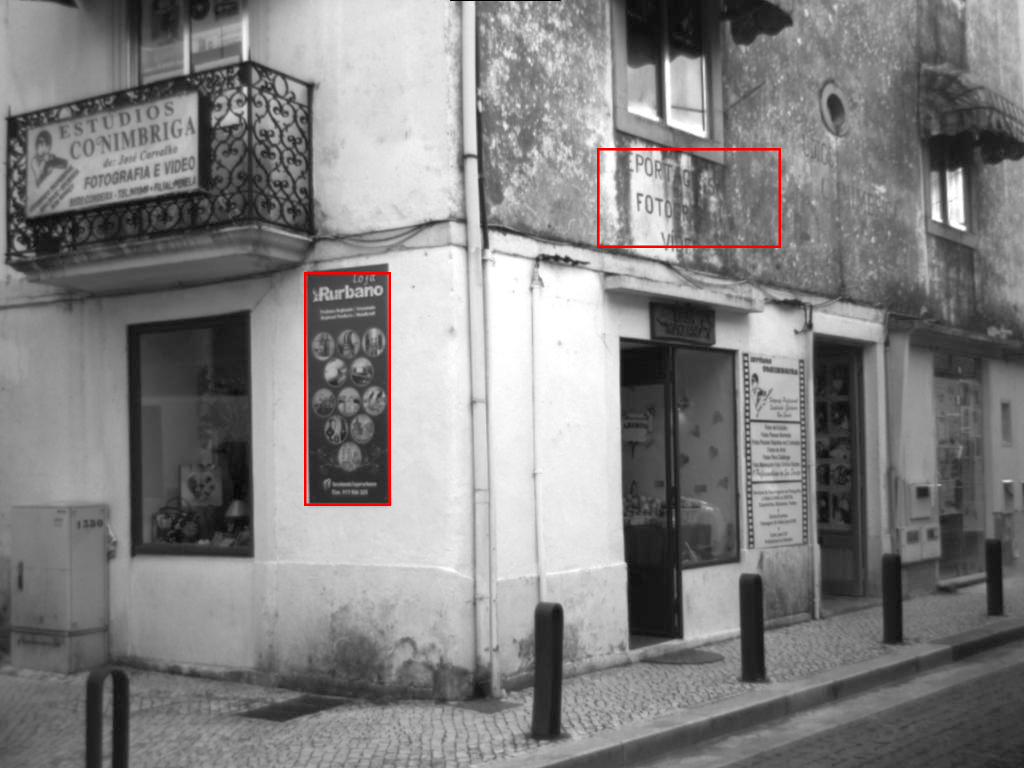
\includegraphics[width=0.80\textwidth]{./images/rectified_stereo_image/original_template_img_with_box.png}
	} \\
	\subfloat[Target image]{
		\label{fig:tar}
		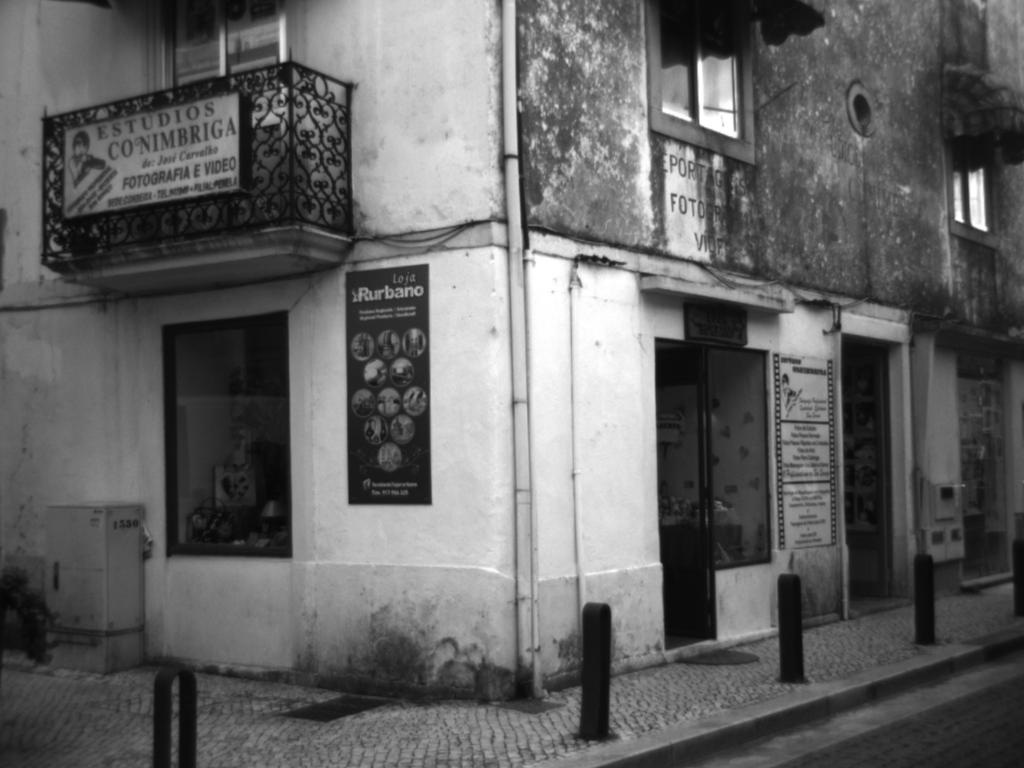
\includegraphics[width=0.80\textwidth]{./images/rectified_stereo_image/original_target_img.png}}
	\caption{Example of a rectified stereo image pair }
	\label{fig:Example rectified stereo images}
\end{figure}

Before running the program, an initialization of parameter $\vec{\beta}_n$ is needed. $a$ and $b$ will start with $1$ and $0$. The reason is that the radiometric distortion is not too much, $a$ and $b$ could start with no radiometric distortion. Parameter $\vec{q}_n$ is initialized as $(0, 0, q_{n_3})$, where $q_{n_3}$ was estimated by hand. In a future version of the algorithm this will be automated.

After initializing $\beta_n$, it is used to warp plane patch $n$ in the target image to the template image, the result of the first plane patch (billboard on the left wall) is shown in \cref{fig:billoadnleft}. Among them, \cref{fig:ddiffBill} shows the difference of this two image patches. It is built by subtract the gray value of the corresponding point. And the difference will be used as gray value of this position to build the difference image. Because the difference of most of pixels is too small, the value is re-scaled by a factor (It's 50 in the thesis) to make it more obvious. What's more, $ difference = I_2 - I_1$ and it is shown in blue for positive value and in red for negative value. 
\begin{figure}[tbp]\centering
	\subfloat[Template image ]{
				\label{fig:temBidll}
		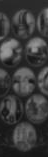
\includegraphics{./images/rectified_stereo_image/patch_2_ROI_of_template.png}
	} \quad
	\subfloat[Warped image]{
				\label{fig:wardpBill}
		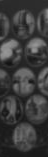
\includegraphics{./images/rectified_stereo_image/patch_2_ROI_of_warped_image.png}
	} \quad
	\subfloat[Difference image]{
				\label{fig:ddiffBill}
		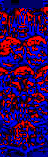
\includegraphics{./images/rectified_stereo_image/patch_2_difference.png}
	} \quad
	\subfloat[]{
		\label{fig:difadfBill}
		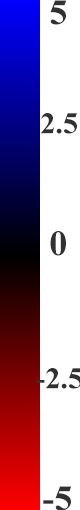
\includegraphics[height = 5.5cm]{./images/legendH}
	} 
	\caption{Result of plane patch of billboard on the left wall }
	\label{fig:billoadnleft}
\end{figure}
%
%\begin{figure}[tbp]\centering
%	\subfloat[Billboard on left balcony in template image ]{
%		\label{fig:temBill}
%		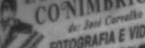
\includegraphics{./images/rectified_stereo_image/patch_1_ROI_of_template.png}
%	} \qquad
%	\subfloat[Billboard on left balcony in warped image]{
%		\label{fig:warpBill}
%		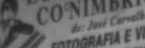
\includegraphics{./images/rectified_stereo_image/patch_1_ROI_of_warped_image.png}
%	} \\
%	\subfloat[Difference image of billborad on left balcony]{
%		\label{fig:diffBill}
%		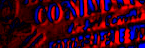
\includegraphics[width = 0.4\textwidth]{./images/rectified_stereo_image/patch_1_difference.png}
%	} \\
%	\subfloat[Legend]{
%		\label{fig:Legend1}
%		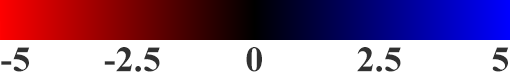
\includegraphics[width = 0.4 \textwidth]{./images/legendW}
%	} 
%	\caption{Result of plane patch of billboard on left balcony}
%	\label{fig:billonbal}
%\end{figure}
And the result of the word on right wall is shown in \cref{fig:word}

\begin{figure}[tbp]\centering
	\subfloat[Word on right wall in template image ]{
%		\label{fig:temBill}
		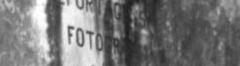
\includegraphics[width = 0.5\textwidth]{./images/rectified_stereo_image/patch_3_ROI_of_template.png}
	} \\
	\subfloat[Word on right wall in warped image]{
%		\label{fig:warpBill}
		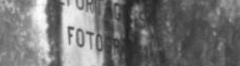
\includegraphics[width = 0.5\textwidth]{./images/rectified_stereo_image/patch_3_ROI_of_warped_image.png}
	} \\
	\subfloat[Difference image of Word on right wall]{
%		\label{fig:diffBill}
		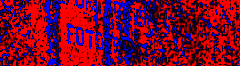
\includegraphics[width = 0.5\textwidth]{./images/rectified_stereo_image/patch_3_difference.png}
	} \\
	\subfloat[Legend]{
	%		\label{fig:diffBill}
	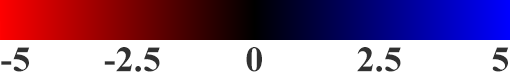
\includegraphics[width = 0.5\textwidth]{./images/legendW}
	} 
	\caption{Result of plane patch of word on right wall}
	\label{fig:word}
\end{figure}

In order to quantify the accuracy of result, the definition of PSNR should be introduced here.(Here the formula of PSNR is used but it doesn't have the meaning for noise, so that the result is not an actual PSNR.)

\begin{definition}[Peak signal-to-noise ratio]\label{def:PSNR}
	Peak signal-to-noise ratio, often abbreviated \\ PSNR, is an engineering term for the ratio between the maximum possible power of a signal and the power of corrupting noise that affects the fidelity of its representation. Because many signals have a 
	very wide dynamic range, PSNR is usually expressed in terms 
	of the logarithmic decibel scale \cite{PeakSignaltonoiseRatio2020}
	
	PSNR is most easily defined via the mean squared error (MSE). Given a noise-free m×n monochrome image I and its noisy approximation K, MSE is defined as:
	\begin{align}
		\mathit{MSE} = \frac{1}{m\,n}\sum_{i=0}^{m-1}\sum_{j=0}^{n-1} [I(i,j) - K(i,j)]^2
	\end{align}
	The PSNR (in dB) is defined as:
	\begin{align}
	\mathit{PSNR} &= 10 \cdot \log_{10} \left( \frac{\mathit{MAX}_I^2}{\mathit{MSE}} \right)\nonumber \\ 
	&= 20 \cdot \log_{10} \left( \frac{\mathit{MAX}_I}{\sqrt{\mathit{MSE}}} \right)\nonumber \\ 
	&= 20 \cdot \log_{10} \left( {\mathit{MAX}_I} \right) - 10 \cdot \log_{10} \left( {{\mathit{MSE}}} \right)
	\end{align}
	Here, MAXI is the maximum possible pixel value of the image. When the pixels are represented using 8 bits per sample, this is 255.
\end{definition}

PSNR is most commonly used to measure the similarity of corresponding images. The PSNR of these three patches is shown in \cref{tab:PSNR of different patches}. The typical value for the PSNR for image registration are between $30$ and $50$ dB, provided the bit depth is $8$ bits, where higher is better. As the difference images show, the results are good, but not perfect. The reason is that the example image is not perfect rectified, so optimization of $H_\infty$ and $\rde$ is also needed, just as what is done in next section.

%And the second patch is relatively not very good, shown in the difference image, there are more deep red pixels. The probably reason is that the image is not perfect rectified, so I need to not only optimize $\vec{q}_n$ but also optimize $H_\infty$ and $\rde$. What's more, there are much noise in the original image, in order to reduce the impact of noise, I also blur the image. The implementation result with optimization is shown in \cref{fig:Result of plane patch of word on billboard on left balcony after optimization}.

%\begin{figure}[tbp]\centering
%	\subfloat[Billboard on left balcony in template image]{
%		%		\label{fig:temBill}
%		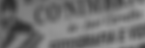
\includegraphics[width = 0.4\textwidth]{./images/rectified_stereo_image/patch_1_of_cycle_6_ROI_of_template}
%	} 
%	\subfloat[Billboard on left balcony in warped image ]{
%		%		\label{fig:warpBill}
%		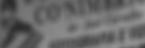
\includegraphics[width = 0.4\textwidth]{./images/patch_1_of_cycle_6_ROI_of_warped_image}
%	} 
%	\caption{Result of plane patch of word on billboard on left balcony after optimization $H_\infty$ and $\rde$}
%	\label{fig:Result of plane patch of word on billboard on left balcony after optimization}
%\end{figure}

\begin{table}[tbp]
	\centering
	\scriptsize  
	\begin{tabular}{p{120pt} p{60pt}}
		\toprule
		Patch & {\bfseries PSNR(dB)}\\ \midrule
		 Billboard on the left wall  &  35.8293\\
		\addlinespace[3pt]
		Word on right wall & 32.0190 \\ \bottomrule
	\end{tabular}
	\caption{PSNR of different patches for rectified images}  
	\label{tab:PSNR of different patches} 
\end{table}

\subsection{Unrectified Images}\label{subsec:Unrectified Images}
Research is extended from special cases to general cases. In last section, the result of the algorithm on rectified stereo images is shown. Next, the algorithm will be applied to normal case, unrectified images, which appears more often in the practical applications. There is no special parameters for normal case, so the whole iterative process shown in \cref{fig:optimized iterative process} will be implemented. The process is divided into two parts: Optimize $\vec{Q}^k, \vec{R}^k$ per patch separately with constant $H_\infty^{(k)}, \rde^{(k)}$ and Optimize $H_\infty^{(k)}, \rde^{(k)}$ for all patches with constant $\vec{Q}^{(k)}, \vec{R}^{(k)}$, where $\vec{Q}^{(k)} = (\vec{q}_1^T, \vec{q}_2^T, \cdots, \vec{q}_n^T)^T$ and $\vec{R}^{(k)}= (\vec{r}_1^T, \vec{r}_2^T, \cdots, \vec{r}_n^T)^T$ with $\vec{r}_n^T= ({r_n}_1, {r_n}_2)$. The first steps Optimize $\vec{Q}^k, \vec{R}^{(k)}$  will be done just like the process in \cref{subsec:Rectified Stereo Images}, the only difference is that $H_\infty^k$ and $\rde^k$ are not always $I_3$ and $(1, 0, 0)^T$ but result of the last iterative process $H_\infty^{k}, \rde^k$. 

So in this section, we will mainly discuss the second part. Detailed calculation process for the second part is shown next. After the step Optimize $\vec{Q}^k, \vec{R}^{(k)}$, the $\vec{q}_n^T$ and $\vec{r}_n^T$ for all patches are got and can be regarded as constant values in this step. So there are only parameter $H_\infty$ and $\rde$ to be optimized. The $\vec{\beta}$ (\cref{eq:beta}) becomes 
\begin{align}
	\vec{\beta} =  \begin{pmatrix}\operatorname {vec}(H_\infty)\\\rde\end{pmatrix}
\end{align}
the Jacobian matrix $\mathbf{J}_{F_n}$ for patch n: 
\begin{align}
	\mathbf{J}_{F_n} = \begin{pmatrix}
	\frac{\mathrm{d} I_2(N)}{\mathrm{d}N} \cdot \frac{\mathrm{d} N(T_n)}{\mathrm{d} T_n} \cdot \frac{\partial T_n(H_\infty, \rde, \rdx_{11})}{\partial \operatorname {vec}(H_\infty)} & \frac{\mathrm{d} I_2(N)}{\mathrm{d}N} \cdot \frac{\mathrm{d} N(T_n)}{\mathrm{d} T_n} \cdot \frac{\partial T_n(H_\infty, \rde, \rdx_{11})}{\partial \rde} \\
	\frac{\mathrm{d} I_2(N)}{\mathrm{d}N} \cdot \frac{\mathrm{d} N(T_n)}{\mathrm{d} T_n} \cdot \frac{\partial T_n(H_\infty, \rde, \rdx_{12})}{\partial \operatorname {vec}(H_\infty)} & \frac{\mathrm{d} I_2(N)}{\mathrm{d}N} \cdot \frac{\mathrm{d} N(T_n)}{\mathrm{d} T_n} \cdot \frac{\partial T_n(H_\infty, \rde, \rdx_{12})}{\partial \rde} \\
	\vdots & \vdots \\
	\frac{\mathrm{d} I_2(N)}{\mathrm{d}N} \cdot \frac{\mathrm{d} N(T_n)}{\mathrm{d} T_n} \cdot \frac{\partial T_n(H_\infty, \rde, \rdx_{ij})}{\partial \operatorname {vec}(H_\infty)} & \frac{\mathrm{d} I_2(N)}{\mathrm{d}N} \cdot \frac{\mathrm{d} N(T_n)}{\mathrm{d} T_n} \cdot \frac{\partial T_n(H_\infty, \rde, \rdx_{ij})}{\partial \rde} \\
	\end{pmatrix}
\end{align}
where $\rdx_{ij} = (\rdx'_{ij}, 1)^T$ and $\rdx_{ij}$ means the $i$ row $j$ column in every patch. They are not the same for different patches. Combine all $\mathbf{J}_{F_n}$, the total $\mathbf{J}_{F}$ is
\begin{align}\label{eq:J_F}
	\mathbf{J}_{F} = \begin{pmatrix} \mathbf{J}_{F_1}\\
	\mathbf{J}_{F_2}\\
	\vdots\\
	\mathbf{J}_{F_n} 
	\end{pmatrix}
\end{align}
The total $\mathbf{J}_{F}$ matrix can be calculated explicit by bringing $\frac{\mathrm{d} N(T_n)}{\mathrm{d} T_n}$ (\cref{eq:n}), $\frac{\partial T_n(H_\infty, \rde, \rdx_{ij})}{\partial \operatorname {vec}(H_\infty)}$ (\cref{eq:H_infty2}) and $ \frac{\partial T_n(H_\infty, \rde, \rdx_{ij})}{\partial \rde}$ (\cref{eq:e1}) into the equation above.

The next step is calculating the total mapping error $\vec{E}$. Just like mentioned in \cref{subsec:Rectified Stereo Images} (\cref{eq:e_n2}), the mapping error $\vec{e}_n$ can be expressed as
\begin{align}
\vec{e}_{n} = \begin{pmatrix} 
	R_n(I_1(N(\rdx_{11})))-F_n(H_\infty, \rde, \rdx_{11})\\
	R_n(I_1(N(\rdx_{12})))-F_n(H_\infty, \rde, \rdx_{12})\\
	\vdots\\
	R_n(I_1(N(\rdx_{ij})))-F_n(H_\infty, \rde, \rdx_{ij})
\end{pmatrix}
\end{align}
Put all $\vec{e}_{n}$ together in $\vec{E}$:
\begin{align}
	\vec{E} = \begin{pmatrix} 
	\vec{e}_{1}\\
	\vec{e}_{2}\\
	\vdots\\
	\vec{e}_{n}
	\end{pmatrix}
\end{align}

Finally $\vec{\beta}$ is iteratively optimized by 
\begin{align}
	\vec{\beta}^{(k+1)} = \vec{\beta}^{(k)} + \left(\mathbf{J}_{F}^{T} \mathbf{J}_{F} \right)^{-1} \mathbf{J}_{F}^{T} \vec{E}
\end{align}

The next step is to implement the algorithm in Python and apply it to example unrectified stereo images. The algorithm will be evaluated on synthetic test images for which the ground truth is available. The details are shown in \cref{sec:Self-Built Datasets}. The template image $I_1$ and target image $I_2$ are shown in \cref{fig:Example unrectified images}. There are three planes in the image, which show a deer, a bouquet of flowers and a cat. Therefore I simply call them deer plane, flower plan and cat plane. 

\begin{figure}[htbp]\centering
	\subfloat[Template image]{
		\label{fig:tem_un}
		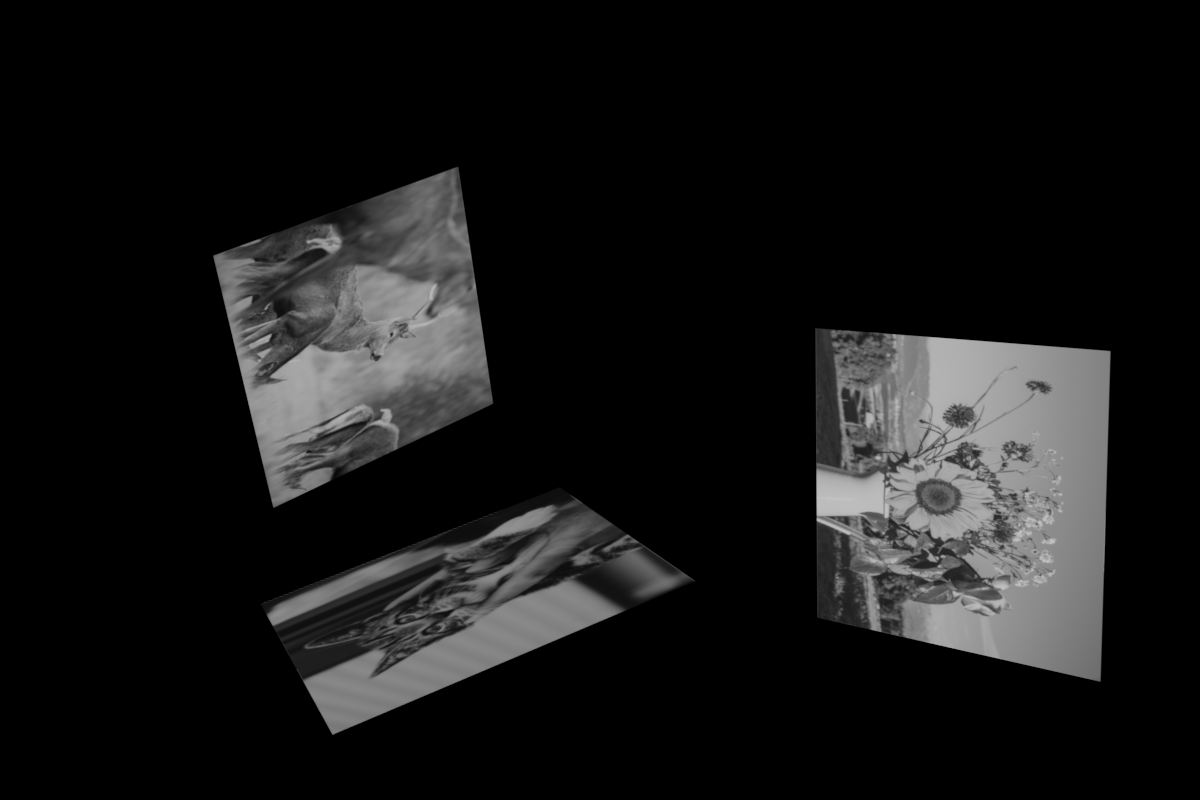
\includegraphics[width=0.80\textwidth]{./images/unrectified_images/original_template_img}
	} \\
	\subfloat[Target image]{
		\label{fig:tar_un}
		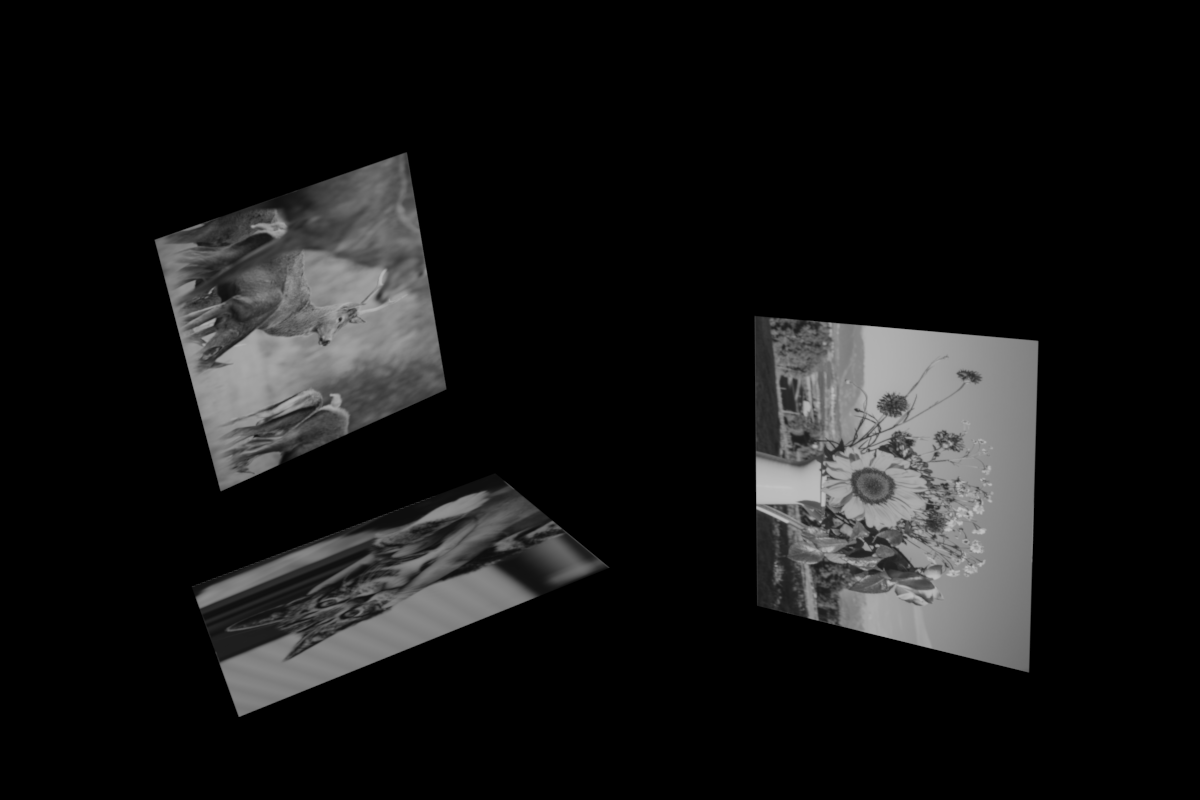
\includegraphics[width=0.80\textwidth]{./images/unrectified_images/original_target_img}}
	\caption{Example unrectified images}
	\label{fig:Example unrectified images}
\end{figure}

Because the testing image pair is synthetically generated, the ground truth is available as well. I will use them to have a good initialization of parameters $H_\infty$, $\rde$ and $\vec{Q}$, which could also be got with the GPS and INS information or EXIF data in practical application.

Just like what is done for rectified stereo images, the final result $H_\infty$, $\rde$, $\vec{Q}$ and $R$ are used to warp the target image to the template image shown in \cref{fig:Result of Unrectified Images}. And the PSNR is shown in \cref{tab:PSNR of different patches in unrectified images}. In order to evaluate the result of the proposed algorithm, the root mean squared displacement (RMSD) is introduced here. 

\begin{definition}[Root mean squared displacement]\label{def:RMSD}
	Because we know the ground truth (homography matrices of different regions of interest ${H_n}_{gt}$) of the self-built image pairs. The ground truth target ${\rdy'_{ij}}_{gt}= N({H_n}_{gt} \cdot \rdx_{ij})$ can be calculated. Then the position $\rdy'_{ij}$ of warped point can be calculated with the estimated homography matrices $H_n$:
	\begin{align}
		\rdy'_{ij} = N(H_n \cdot \rdx_{ij})
	\end{align}

	Root mean squared displacement (RMSD) is defined as
	\begin{align}
	\mathrm{RMSD} & = \sqrt{\frac{1}{n}\sum_{\rdx_{ij}\in ROI} \|\rdy'_{ij} - {\rdy'_{ij}}_{gt} \|^2}
	\end{align}
	where $n$ means the number of points in the region of interest (patches) and $\|\rdy'_{ij} - {\rdy'_{ij}}_{gt} \|$ is the distance $d$ between tow points. RMSD is the measure of the average distance between two vector space, here means how much the difference between the estimated result and ground truth.
\end{definition}
	
The root mean squared displacement (RMSD) and maximum displacement of all patches are shown in \cref{tab:Displacement of different patches for unrectified images}. From the difference images, we can see visually that there is basically no difference. From the PSNR analysis, the value is relatively high. So the result is acceptable. And because the whole parameters are optimized, there are no large matching error as in the rectified case (\cref{fig:word})
\begin{figure}[htbp]\centering
	\subfloat[Template image]{
		\label{fig:Template Image1}
		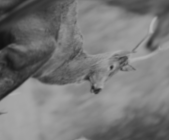
\includegraphics[width=0.30\textwidth]{images/unrectified_images/patch_1_of_cycle_1_ROI_of_template}
	}  \hspace{-2mm}
	\subfloat[Warped image for deer plane]{
		\label{fig:Warped Image For Deer Plane}
		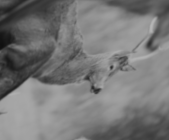
\includegraphics[width=0.30\textwidth]{images/unrectified_images/patch_1_of_cycle_1_ROI_of_warped_image}
	} \hspace{-2mm}
	\subfloat[Difference image]{
		\label{fig:Difference Image1}
		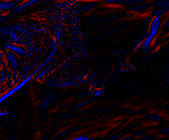
\includegraphics[width=0.30\textwidth]{images/unrectified_images/patch_1_difference}
	}\hspace{-2.5mm}
	\subfloat[]{
	%		\label{fig:diffBill}
	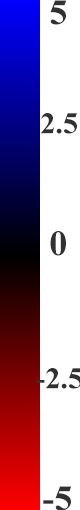
\includegraphics[height = 3.6cm]{./images/legendH}
	} 
	\\

	\subfloat[Template image]{
		\label{fig:Template Image2}
		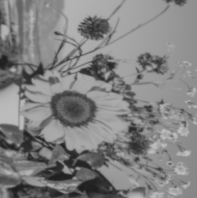
\includegraphics[width=0.30\textwidth]{images/unrectified_images/patch_2_of_cycle_1_ROI_of_template}
	} \hspace{-2mm}
	\subfloat[Warped image for flower plane]{
		\label{fig:Warped Image For Flower Plane}
		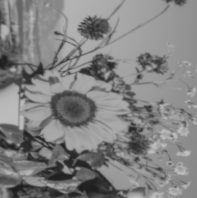
\includegraphics[width=0.30\textwidth]{images/unrectified_images/patch_2_of_cycle_1_ROI_of_warped_image}
	}\hspace{-2mm}
	\subfloat[Difference image]{
		\label{fig:Difference Image2}
		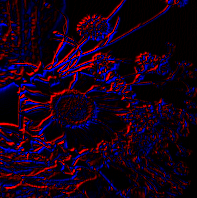
\includegraphics[width=0.30\textwidth]{images/unrectified_images/patch_2_difference}
	}\hspace{-2.5mm}
	\subfloat[]{
	%		\label{fig:diffBill}
	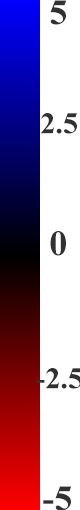
\includegraphics[height = 4.3cm]{./images/legendH}
} 
	\\

	\subfloat[Template image]{
		\label{fig:Template Image3}
		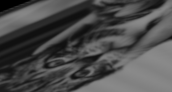
\includegraphics[width=0.30\textwidth]{images/unrectified_images/patch_3_of_cycle_1_ROI_of_template}
	} \hspace{-2mm}
	\subfloat[Warped image for cat plane]{
		\label{fig:Warped Image For Cat Plane}
		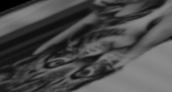
\includegraphics[width=0.30\textwidth]{images/unrectified_images/patch_3_of_cycle_1_ROI_of_warped_image}
	} \hspace{-2mm}
		\subfloat[Difference image]{
		\label{fig:Difference Image3}
		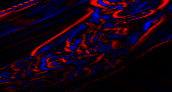
\includegraphics[width=0.30\textwidth]{images/unrectified_images/patch_3_difference}
	}\hspace{-2.5mm}
	\subfloat[]{
	%		\label{fig:diffBill}
	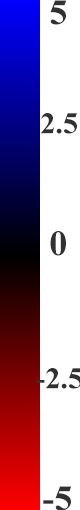
\includegraphics[height = 2.4cm]{./images/legendH}
} 
\\
	\caption{Result of unrectified Images}
	\label{fig:Result of Unrectified Images}
\end{figure}

\begin{table}[htbp]
	\centering
	\scriptsize  
	\begin{tabular}{p{80pt} p{60pt}}
		\toprule
		Patch & {\bfseries PSNR(dB)}\\ \midrule
		Deer Plane&  44.9857\\
		\addlinespace[3pt]
		Flower Plane  &  38.3061\\
		\addlinespace[3pt]
		Cat Plane & 41.5518 \\ \bottomrule
	\end{tabular}
	\caption{PSNR of different patches for unrectified images}  
	\label{tab:PSNR of different patches in unrectified images} 
\end{table}

\begin{table}[htbp]
	\centering
	\scriptsize   
	\begin{tabular}{p{80pt} p{60pt} p{60pt}}
		\toprule
		 Patch & {\bfseries RMSD (pixel)} & {\bfseries Maximum(pixel)}\\ \midrule
		 Deer Plane&  0.186577&0.370456 \\
		 \addlinespace[3pt]
		 Flower Plane  &  0.130046&0.162404 \\
		 \addlinespace[3pt]
		 Cat Plane & 0.369888&0.874363 \\ 
		 \addlinespace[3pt]
		 All Patches & 0.215594&0.874363 \\ \bottomrule
	\end{tabular}
	\caption{Displacement of different patches for unrectified images}  
	\label{tab:Displacement of different patches for unrectified images} 
\end{table}
In this chapter I only show one example result of the algorithm for each case. More results are listed evaluation in \cref{ch:Evaluation}.







